%%%%%%%%%%%%%%%%%%%%%%%%%%%%%%%%%%%%%%%%%%%%%%%%%%%%%%%%%%%%%%%%%%%%%%%%%%%%%%%
% LaTeX Document for WuBu Nesting Paper
% Generated based on WuBuHypCD-paper.md
% Template: Standard Article Class for arXiv
% --- Version 3 Corrections ---
% - Renamed \hyp to \HypSpace
% - Used \url{} for filename formatting (removed hyphenat)
% - Scaled TikZ diagram further
% --- Version 4 Corrections (Based on Compile Log) ---
% - Added \texorpdfstring for math in titles/captions causing hyperref warnings
% - Added \sloppypar around paragraph likely causing overfull hbox
% --- Version 5 Corrections (Based on Compile Log) ---
% - Correctly added $...$ inside first arg of \texorpdfstring for math commands
% - Fixed \texorpdfstring in optional args of \subsubsection
% - Adjusted \sloppypar placement based on new overfull hbox warnings
% --- Version 6 Corrections (Based on Compile Log) ---
% - Removed unnecessary \texorpdfstring from body text (abstract, paragraphs)
% - Ensured all math in body text is correctly delimited with $...$
% - Corrected \texorpdfstring usage in sectioning/captions
% - Removed \sloppypar temporarily to reassess line breaks after error fixes
% --- Version 7 Corrections (Based on Compile Log) ---
% - Re-added \sloppypar for persistent overfull hbox before figure
% - Simplified plain text in \texorpdfstring (removed ^, _) for hyperref warnings
% --- Version 8 Corrections (Based on Compile Log) ---
% - Further simplified plain text in \subsubsection optional arg for hyperref warning
%%%%%%%%%%%%%%%%%%%%%%%%%%%%%%%%%%%%%%%%%%%%%%%%%%%%%%%%%%%%%%%%%%%%%%%%%%%%%%%
\documentclass[11pt, twoside]{article} % Use 11pt font, two-side layout typical for articles

% --- Essential Packages ---
\usepackage[utf8]{inputenc}      % Handle UTF-8 input
\usepackage[T1]{fontenc}       % Use modern font encodings
\usepackage{amsmath, amssymb, amsfonts, amsthm} % AMS packages + theorem environments
\usepackage{graphicx}            % For including figures (still needed if other figs exist)
\usepackage[numbers,sort&compress]{natbib} % For numbered citations, sorted and compressed
\usepackage{hyperref}            % For clickable links and references
\usepackage{geometry}            % For setting page margins
\usepackage{booktabs}            % For professional quality tables (if needed later)
\usepackage{xcolor}              % For potential text coloring (e.g., comments)
\usepackage{float}               % For better figure placement control (e.g., [H])
\usepackage{microtype}           % Improves typography (subtle spacing adjustments)
\usepackage{lmodern}             % Use Latin Modern fonts (often preferred over Computer Modern)
\usepackage{caption}             % For customizing captions
\usepackage{listings}            % For code listings (if needed later)
\usepackage{enumitem}            % For customized lists
% \usepackage[htt]{hyphenat}     % Removed - caused issues, use \url instead

% --- TikZ Package and Libraries for Diagram ---
\usepackage{tikz}
\usetikzlibrary{shapes.geometric, arrows.meta, positioning, calc, fit, decorations.pathreplacing}

% --- Page Geometry ---
% Standard margins suitable for arXiv
\geometry{
    letterpaper,
    top=1in,
    bottom=1in,
    left=1in,
    right=1in,
}

% --- Hyperref Setup ---
% Use \texorpdfstring ONLY for commands that might go into bookmarks AND contain problematic LaTeX
\hypersetup{
    colorlinks=true,
    linkcolor=blue!70!black,       % Slightly darker blue for links
    citecolor=green!60!black, % Slightly darker green for citations
    filecolor=magenta,
    urlcolor=cyan!70!black,
    pdftitle={WuBu Nesting: A Comprehensive Geometric Framework for Adaptive Multi-Scale Hierarchical Representation with Integrated Rotational Dynamics}, % Title is okay as plain text
    pdfauthor={WaefreBeorn}, % IMPORTANT: Update this
    pdfsubject={Geometric Deep Learning, Hyperbolic Geometry, Machine Learning},
    pdfkeywords={Hyperbolic Geometry, Geometric Deep Learning, Nested Models, Rotation, Tangent Space, Hierarchy, Representation Learning},
    bookmarksopen=true,
    bookmarksnumbered=true,
    breaklinks=true % Allow links to break across lines
}

% --- Bibliography Style ---
\bibliographystyle{plainnat} % Standard numerical style

% --- Custom Commands (Optional) ---
% Definition now includes $...$ internally. Use directly in text.
% \texorpdfstring is only needed if this command itself is used in a bookmark-generating context (like \section)
% which is unlikely for a complex command like this. We rely on hyperref handling simple math in bookmarks.
\newcommand{\HypSpaceCmd}[3]{\mathcal{H}^{#1}_{#2, #3}} % Raw command for math mode
% Simplified plain text version for bookmarks (removed ^ and _)
\newcommand{\HypSpace}[3]{\texorpdfstring{$\HypSpaceCmd{#1}{#2}{#3}$}{H{#1}{#2}{#3}}} % Command for use in bookmarks if needed

\newcommand{\tangentCmd}[2]{T_{#1}(\mathcal{H}^{#2})} % Raw command for math mode
% Simplified plain text version for bookmarks (removed ^ and _)
\newcommand{\tangent}[2]{\texorpdfstring{$\tangentCmd{#1}{#2}$}{T{#1}(H{#2})}} % Command for use in bookmarks if needed

\newcommand{\R}{\mathbb{R}} % Real numbers symbol
\newcommand{\SOcmd}[1]{\text{SO}(#1)} % Raw command for math mode
\newcommand{\SO}[1]{\texorpdfstring{$\SOcmd{#1}$}{SO(#1)}} % Command for use in bookmarks if needed

\newcommand{\wubu}{\textbf{WuBu Nesting}} % Consistent naming

% --- TikZ Styles ---
\tikzstyle{block} = [rectangle, draw, thick, text centered, rounded corners, minimum height=2.2em, text width=6.5em, fill=gray!5]
\tikzstyle{data} = [ellipse, draw, thick, text centered, minimum height=2.2em, fill=blue!5]
\tikzstyle{process} = [block, fill=green!10, draw=green!50!black]
\tikzstyle{transform} = [block, fill=orange!15, draw=orange!70!black]
\tikzstyle{rotation} = [block, fill=yellow!20, draw=yellow!70!black]
\tikzstyle{map} = [block, fill=blue!10, draw=blue!50!black]
\tikzstyle{aggregate} = [block, fill=purple!10, draw=purple!60!black]
\tikzstyle{output} = [data, fill=red!10, draw=red!60!black]
\tikzstyle{arrow} = [thick,->,>=Stealth]
\tikzstyle{levelbox} = [draw, thick, dashed, rounded corners, inner sep=10pt, label distance=2mm]
\tikzstyle{smalllabel} = [font=\tiny, text width=2.5cm, align=center] % Style for arrow labels, smaller font

% --- Title, Author, Date ---
% \wubu is bold text, should be fine for title.
\title{\wubu: A Comprehensive Geometric Framework for Adaptive Multi-Scale Hierarchical Representation with Integrated Rotational Dynamics}

% --- IMPORTANT: Replace with actual author names and affiliations ---
\author{
    Wubu WaefreBeorn\thanks{Wubu WaefreBeorn, X: @WaefreBeorn Twitch: @WaefreBeorn Youtube: @WuBuStreams @WaefreBeorn}
    % Add more authors as needed
}
\date{} % Leave blank for arXiv date stamp

%%%%%%%%%%%%%%%%%%%%%%%%%%%%%%%%%%%%%%%%%%%%%%%%%%%%%%%%%%%%%%%%%%%%%%%%%%%%%%%
% Document Start
%%%%%%%%%%%%%%%%%%%%%%%%%%%%%%%%%%%%%%%%%%%%%%%%%%%%%%%%%%%%%%%%%%%%%%%%%%%%%%%
\begin{document}

\maketitle

% --- Abstract ---
% Removed \texorpdfstring, ensured math is delimited with $...$
\begin{abstract}
Real-world data frequently exhibits complex characteristics including multi-scale hierarchical organization, rotational symmetries, dynamic evolution, and regional uncertainty. While geometric deep learning offers powerful tools, existing paradigms often specialize: Euclidean models struggle with hierarchies, hyperbolic models typically handle single static hierarchies without rotational mechanics, and quaternion networks excel at rotation but lack hierarchical structure. To address these limitations, we introduce \wubu{} ("layered nesting"), a novel conceptual framework unifying these geometric properties. \wubu{} employs a recursively nested structure of hyperbolic spaces ($\HypSpaceCmd{n_1}{c_1}{s_1} \supset \HypSpaceCmd{n_2}{c_2}{s_2} \supset \dots$) where dimensionality ($n_i$), curvature ($c_i > 0$), and scale ($s_i > 0$) are learnable, allowing dynamic adaptation to data complexity. Each level $i$ incorporates learnable Boundary Sub-Manifolds representing scale-specific structures. Inter-level transitions ($i \rightarrow i+1$) occur in Euclidean tangent spaces ($T_p(\HypSpaceCmd{n_i}{}{}) \cong \R^{n_i}$), featuring a learned Rotation ($R_i$, e.g., $\SOcmd{n_i}$ or Quaternions) applied simultaneously to primary data, boundary representations, and a learnable Level Descriptor ($\mathbf{ld}_i$). This is followed by a non-rotational Mapping ($\tilde{T}_i$) adjusting features and dimension. Relative Vectors ($\mathbf{d}_{i+1, j, k}$) are computed in the target tangent space, encoding rotation-aware structure. Each level also has a learnable Spread Parameter ($\sigma_i$) for uncertainty context and allows Intra-Level Tangent Flow ($F_i$) for local dynamics. The resulting rich information flow enables \wubu{} to capture intertwined hierarchical, rotational, dynamic, and uncertain characteristics, offering a highly flexible geometric inductive bias for complex data modeling.
\end{abstract}

% --- Main Body Sections ---

\section{Introduction}
\label{sec:introduction}

Effective data representation is fundamental to machine learning. While standard deep learning models achieve remarkable success, their predominant reliance on Euclidean geometry limits their ability to capture intrinsic data structures not naturally suited to flat spaces. Hierarchical data---taxonomies, phylogenetic trees, molecular structures, articulated objects, parse trees---presents a key challenge. Embedding hierarchies in Euclidean space incurs significant distortion due to the mismatch between Euclidean polynomial volume growth and the typically exponential expansion of hierarchical nodes \cite{NickelKiela2017}.

Hyperbolic geometry, with its constant negative curvature and exponential volume growth, provides a more natural embedding space for such structures \cite{NickelKiela2017, KhrulkovEtAl2020, ErmolovEtAl2022}. Models utilizing the Poincaré ball ($\mathcal{H}^n$) or other hyperbolic models have shown substantial advantages in graph embedding, NLP \cite{GaneaEtAl2018, GulcehreEtAl2019}, computer vision \cite{KhrulkovEtAl2020, ErmolovEtAl2022, AtighEtAl2022}, and category discovery \cite{LiuHeHan2025}, demonstrating the benefit of aligning geometric inductive bias with data structure.

However, real-world systems often exhibit complexities beyond single, static hierarchies. Data frequently possesses \textbf{nested hierarchies} (structures within structures) and involves components with \textbf{intrinsic orientations} where transformations between levels or viewpoints include \textbf{rotations}. For instance, modeling articulated objects requires understanding both part hierarchies and their relative rotational movements. Existing hyperbolic models typically focus on a single hierarchy level with fixed geometry, lacking mechanisms for adaptive multi-scale nesting or integrated rotational modeling.

Conversely, Quaternions \cite{Hamilton1866} offer efficient rotation representation, leveraged by Quaternion Neural Networks (QNNs) \cite{ParcolletEtAl2019, GrassucciEtAl2021} for tasks involving orientation. However, QNNs operate in Euclidean spaces, lacking intrinsic hierarchical embedding capabilities. Product manifolds ($\R^n \times S^m \times \mathcal{H}^k$) \cite{GuEtAl2019} combine geometries in parallel but do not directly model nested structures or integrated inter-level rotational transformations.

This paper introduces \textbf{\wubu{}}, a comprehensive conceptual framework designed to bridge these gaps by unifying adaptive multi-scale hierarchical representation with explicit modeling of rotational dynamics, dynamic evolution, and regional uncertainty. Instead of a single space or parallel product, \wubu{} proposes a nested "Russian doll" architecture of recursively embedded hyperbolic manifolds. Key innovations include:

% Removed \texorpdfstring from list items, ensured math is delimited with $...$
\begin{enumerate}[label=\arabic*), wide, labelindent=0pt]
    \item \textbf{Adaptive Nested Hyperbolic Geometry:} A sequence of nested hyperbolic spaces $\HypSpaceCmd{n_1}{c_1}{s_1} \supset \HypSpaceCmd{n_2}{c_2}{s_2} \supset \dots$, where dimensionality $n_i$, curvature $c_i > 0$, and scale $s_i > 0$ are learnable, allowing dynamic geometric adaptation.
    \item \textbf{Boundary Sub-Manifolds:} Learnable manifolds $B_{i,j}$ within each level $\HypSpaceCmd{n_i}{}{}$ (e.g., parameterized by points $\{\mathbf{b}_{i,j,k}\}$) representing scale-specific substructures or landmarks.
    \item \textbf{Tangent Space Transitions:} Inter-level transitions ($i \rightarrow i+1$) mediated within Euclidean tangent spaces $T_p(\HypSpaceCmd{n_i}{}{}) \cong \R^{n_i}$, enabling complex yet tractable transformations.
    \item \textbf{Explicit Tangent Space Rotations ($R_i$):} A learnable rotation $R_i$ (e.g., $\SOcmd{n_i}$ or Quaternions) applied within $T_o(\HypSpaceCmd{n_i}{}{})$.
    \item \textbf{Simultaneous Transformation:} Rotation $R_i$ applied consistently to the main tangent vector $\mathbf{v}_i$, boundary tangent vectors $\mathbf{v}_{b_{i,j,k}}$, and a learnable Level Descriptor Vector $\mathbf{ld}_i$.
    \item \textbf{Non-Rotational Mapping ($\tilde{T}_i$):} A learnable mapping $\tilde{T}_i: T_o(\HypSpaceCmd{n_i}{}{}) \rightarrow T_o(\HypSpaceCmd{n_{i+1}}{}{})$ following rotation, handling feature transformation and dimension changes. Full tangent transform: $T_{i \rightarrow i+1} = \tilde{T}_i \circ R_i$.
    \item \textbf{Relative Vector Generation ($\mathbf{d}_{i+1}$):} Computed in the target tangent space $T_o(\HypSpaceCmd{n_{i+1}}{}{})$ as $\mathbf{d}_{i+1, j, k} = \mathbf{v}_{i+1} - \mathbf{v}''_{b_{i,j,k}}$, encoding rotation-aware structure.
    \item \textbf{Learnable Level Descriptor Vector ($\mathbf{ld}_i$):} An intrinsic vector $\mathbf{ld}_i \in T_o(\HypSpaceCmd{n_i}{}{})$ capturing level-specific geometric properties, transformed to $\mathbf{ld}_{i+1}$ for the next level.
    \item \textbf{Learnable Level Spread Parameter ($\sigma_i$):} A scalar $\sigma_i > 0$ representing scale-specific uncertainty or density, passed as context to level $i+1$.
    \item \textbf{Intra-Level Tangent Flow ($F_i$):} A learnable field $F_i: T_o(\HypSpaceCmd{n_i}{}{}) \rightarrow T_o(\HypSpaceCmd{n_i}{}{})$ modeling dynamics or adjustments within level $i$.
    \item \textbf{Rich Hierarchical Information Flow:} Level $i+1$ processing uses the primary representation, relative vectors $\{\mathbf{d}_{i+1, j, k}\}$, transformed descriptor $\mathbf{ld}_{i+1}$, and contextual spread $\sigma_i$.
\end{enumerate}

We posit that this integrated geometric structure provides a powerful and flexible inductive bias for modeling complex real-world systems exhibiting intertwined hierarchical, rotational, dynamic, and uncertain characteristics.

\section{Related Work}
\label{sec:related_work}

The \wubu{} framework builds upon and synthesizes concepts from several areas of geometric deep learning.

\subsection{Hyperbolic Deep Learning}
\label{subsec:hyperbolic_dl}

Pioneered by Nickel and Kiela \cite{NickelKiela2017}, hyperbolic geometry offers superior embedding for hierarchical data compared to Euclidean spaces due to its negative curvature and exponential volume growth. Subsequent work extended this to tree embeddings \cite{KhrulkovEtAl2020}, graph embeddings \cite{ErmolovEtAl2022, ChamiEtAl2019, ZhangEtAl2021}, ontologies \cite{AtighEtAl2022}, hyperbolic neural network operations \cite{GaneaEtAl2018, GulcehreEtAl2019}, and applications in computer vision \cite{KhrulkovEtAl2020, ErmolovEtAl2022, AtighEtAl2022, LiuHeHan2025}.

\textbf{Critique \& WuBu Distinction:} Existing methods typically use a single, fixed-curvature hyperbolic space. They lack mechanisms for adaptive nested hierarchies and explicit rotational modeling. \wubu{} introduces learnable, nested geometries ($n_i, c_i, s_i$), boundary manifolds, level descriptors, spread parameters, tangent flows, and integrated rotation-aware tangent space transitions.

\subsection{Quaternion Neural Networks (QNNs)}
\label{subsec:qnn}

QNNs \cite{ParcolletEtAl2019, GrassucciEtAl2021} leverage the efficiency of quaternions \cite{Hamilton1866} for representing 3D/4D rotations, achieving parameter efficiency and respecting rotational symmetries in tasks like 3D vision and robotics.

\textbf{Critique \& WuBu Distinction:} QNNs operate in Euclidean spaces and lack intrinsic hierarchical embedding capabilities. \wubu{} integrates rotational modeling (potentially via quaternions) within tangent space transitions between nested hyperbolic levels, combining rotational awareness with adaptive hierarchy.

\subsection{Product Manifolds and Multi-Scale Approaches}
\label{subsec:product_multiscale}

Product manifolds \cite{GuEtAl2019} (e.g., $\R^n \times S^m \times \mathcal{H}^k$) combine different geometries in parallel, increasing capacity but lacking nested structure and sophisticated inter-geometry transformations. Traditional multi-scale methods (e.g., feature pyramids) operate in Euclidean space without specific geometric biases for hierarchy or rotation.

\textbf{Critique \& WuBu Distinction:} \wubu{} proposes a fundamentally different recursive embedding architecture, not parallel composition. Its inter-level transitions are designed to be geometrically meaningful, incorporating learned rotations and mappings, unlike the simpler aggregation often used in product spaces. It integrates hierarchy, scale, rotation, dynamics, and uncertainty in a unified framework distinct from standard multi-scale techniques.

\section{The WuBu Nesting Framework}
\label{sec:framework}

\wubu{} provides a recursive, multi-level geometric architecture. Data flows through nested hyperbolic spaces, with inter-level transitions orchestrated in tangent spaces, incorporating rotations, mappings, relative vector generation, and propagation of level-specific context (descriptors, spread).

\subsection{Conceptual Architecture}
\label{subsec:conceptual_architecture}

% Re-added \sloppypar for overfull hbox reported at lines 302-304
\begin{sloppypar}
Input data is initially encoded and mapped to the tangent space of the outermost level ($\HypSpaceCmd{n_1}{c_1}{s_1}$). Within level $i$, processing occurs, potentially including intra-level tangent flow $F_i$. For transition $i \rightarrow i+1$, the primary representation, boundary manifold representations $\{\mathbf{b}_{i,j,k}\}$, and level descriptor $\mathbf{ld}_i$ are mapped to tangent vectors ($\mathbf{v}_i^{\text{out}}, \{\mathbf{v}_{b_{i,j,k}}\}, \mathbf{ld}_i^{\text{param}}$) via $\text{Log}_{o,s_i}^{c_i}$. A rotation $R_i$ is applied simultaneously to these vectors in $T_o(\HypSpaceCmd{n_i}{}{})$. A mapping $\tilde{T}_i$ then transforms the rotated vectors into the target tangent space $T_o(\HypSpaceCmd{n_{i+1}}{}{})$, yielding $\mathbf{v}_{i+1}, \{\mathbf{v}''_{b_{i,j,k}}\}, \mathbf{ld}_{i+1}$. Relative vectors $\mathbf{d}_{i+1, j, k} = \mathbf{v}_{i+1} - \mathbf{v}''_{b_{i,j,k}}$ are computed. Level $i+1$ processing uses $\mathbf{v}_{i+1}$ (often mapped to $\mathbf{x}_{i+1}$ via $\text{exp}_{o,s_{i+1}}^{c_{i+1}}$), relative vectors $\{\mathbf{d}_{i+1, j, k}\}$, descriptor $\mathbf{ld}_{i+1}$, and spread $\sigma_i$ from level $i$. Aggregated information from relevant levels forms the final output. (See Figure \ref{fig:architecture_tikz}).
\end{sloppypar}

% --- TikZ Diagram ---
% Scaled down further to fit page better
\begin{figure}[htbp]
    \centering
    % Added scale=0.58 and transform shape
    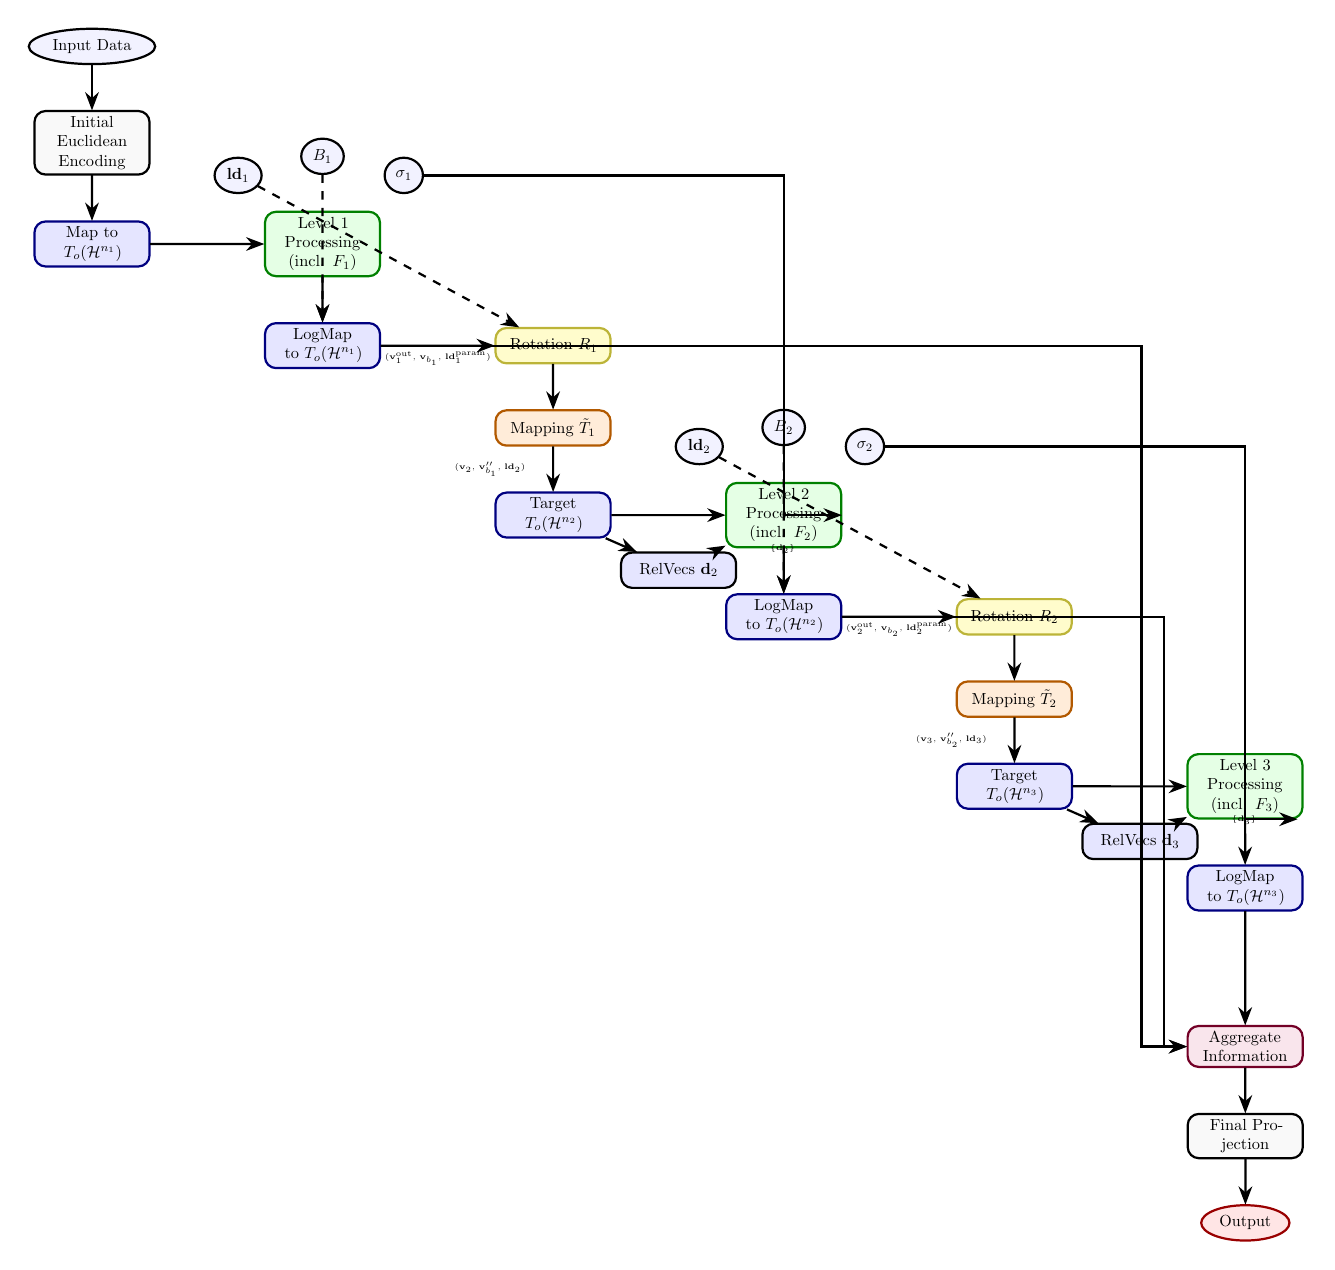
\begin{tikzpicture}[scale=0.58, transform shape, node distance=1.0cm and 1.3cm, auto, >=Latex] % Further reduced scale

        % Nodes - Use math mode $...$ for commands like \mathcal, \mathbf
        \node (input) [data] {Input Data};
        \node (enc) [block, below=of input] {Initial Euclidean Encoding};
        \node (tan1) [map, below=of enc] {Map to $T_o(\mathcal{H}^{n_1})$};

        % Level 1
        \node (proc1) [process, right=2.5cm of tan1] {Level 1 Processing (incl. $F_1$)};
        \node (ld1) [data, above left=0.5cm and 0.2cm of proc1] {$\mathbf{ld}_1$};
        \node (sig1) [data, above right=0.5cm and 0.2cm of proc1] {$\sigma_1$};
        \node (bm1) [data, above=0.8cm of proc1] {$B_1$};
        \node (logmap1) [map, below=of proc1] {LogMap to $T_o(\mathcal{H}^{n_1})$};

        % Transformation 1->2
        \node (rot1) [rotation, right=2.5cm of logmap1] {Rotation $R_1$};
        \node (map1) [transform, below=of rot1] {Mapping $\tilde{T}_1$};
        \node (tan2) [map, below=of map1] {Target $T_o(\mathcal{H}^{n_2})$};
        \node (relvec2) [block, below right=0.3cm and 0.2cm of tan2, fill=blue!10] {RelVecs $\mathbf{d}_2$};

        % Level 2 Processing
        \node (proc2) [process, right=2.5cm of tan2] {Level 2 Processing (incl. $F_2$)};
        \node (ld2) [data, above left=0.5cm and 0.2cm of proc2] {$\mathbf{ld}_2$};
        \node (sig2) [data, above right=0.5cm and 0.2cm of proc2] {$\sigma_2$};
        \node (bm2) [data, above=0.8cm of proc2] {$B_2$};
        \node (logmap2) [map, below=of proc2] {LogMap to $T_o(\mathcal{H}^{n_2})$};

        % Transformation 2->3
        \node (rot2) [rotation, right=2.5cm of logmap2] {Rotation $R_2$};
        \node (map2) [transform, below=of rot2] {Mapping $\tilde{T}_2$};
        \node (tan3) [map, below=of map2] {Target $T_o(\mathcal{H}^{n_3})$};
        \node (relvec3) [block, below right=0.3cm and 0.2cm of tan3, fill=blue!10] {RelVecs $\mathbf{d}_3$};

        % Level 3 (Example - could continue)
        \node (proc3) [process, right=2.5cm of tan3] {Level 3 Processing (incl. $F_3$)};
        \node (logmap3) [map, below=of proc3] {LogMap to $T_o(\mathcal{H}^{n_3})$}; % Output from L3

        % Aggregation & Output (Positioned relative to last level)
        \node (agg) [aggregate, below=2.5cm of logmap3] {Aggregate Information};
        \node (proj) [block, below=of agg] {Final Projection};
        \node (out) [output, below=of proj] {Output};

        % Arrows - Initial Path
        \draw [arrow] (input) -- (enc);
        \draw [arrow] (enc) -- (tan1);
        \draw [arrow] (tan1) -- (proc1);
        \draw [arrow] (proc1) -- (logmap1);

        % Arrows - Level 1 to Transform 1->2
        % Use math mode $...$ for math in node labels
        \draw [arrow] (logmap1) -- node[below, midway, smalllabel] {($\mathbf{v}_1^{\text{out}}$, $\mathbf{v}_{b_1}$, $\mathbf{ld}_1^{\text{param}}$)} (rot1);
        \draw [arrow] (rot1) -- (map1);
        \draw [arrow] (map1) -- node[left, midway, smalllabel] {($\mathbf{v}_2$, $\mathbf{v}''_{b_1}$, $\mathbf{ld}_2$)} (tan2);
        \draw [arrow] (tan2) -- (relvec2);

        % Arrows - Transform 1->2 to Level 2
        \draw [arrow] (tan2) -- (proc2);
        \draw [arrow] (relvec2) -- node[right, midway, smalllabel] {$\{\mathbf{d}_2\}$} (proc2);
        \draw [arrow] (sig1) -| ($(proc2.north) + (0, 0.5cm)$) |- (proc2); % Sigma context path

        % Arrows - Level 2 to Transform 2->3
        \draw [arrow] (proc2) -- (logmap2);
        \draw [arrow] (logmap2) -- node[below, midway, smalllabel] {($\mathbf{v}_2^{\text{out}}$, $\mathbf{v}_{b_2}$, $\mathbf{ld}_2^{\text{param}}$)} (rot2);
        \draw [arrow] (rot2) -- (map2);
        \draw [arrow] (map2) -- node[left, midway, smalllabel] {($\mathbf{v}_3$, $\mathbf{v}''_{b_2}$, $\mathbf{ld}_3$)} (tan3);
        \draw [arrow] (tan3) -- (relvec3);

        % Arrows - Transform 2->3 to Level 3
        \draw [arrow] (tan3) -- (proc3);
        \draw [arrow] (relvec3) -- node[right, midway, smalllabel] {$\{\mathbf{d}_3\}$} (proc3);
        \draw [arrow] (sig2) -| ($(proc3.north) + (0, 0.5cm)$) |- (proc3); % Sigma context path

        % Arrows - Level 3 to Aggregation
        \draw [arrow] (proc3) -- (logmap3);
        \draw [arrow] (logmap3) -- (agg);

        % Arrows - Aggregation from earlier levels (Example)
        \draw [arrow] (logmap1) -| ($(agg.north west) + (-1cm, 1cm)$) |- (agg);
        \draw [arrow] (logmap2) -| ($(agg.west) + (-0.5cm, 0)$) |- (agg);

        % Arrows - Final Path
        \draw [arrow] (agg) -- (proj);
        \draw [arrow] (proj) -- (out);

        % Dashed Arrows (Conceptual Inputs)
        \draw [arrow, dashed] (bm1) -- (logmap1);
        \draw [arrow, dashed] (ld1) -- (rot1);
        \draw [arrow, dashed] (bm2) -- (logmap2);
        \draw [arrow, dashed] (ld2) -- (rot2); % Connect LD2 to Rotation 2

    \end{tikzpicture}
    % Simplified plain text versions in \texorpdfstring for bookmark compatibility
    \caption{Conceptual Architecture of the Comprehensive WuBu Nesting Framework (TikZ Diagram). Illustrates data flow through nested hyperbolic levels (\texorpdfstring{$\HypSpaceCmd{n_i}{c_i}{s_i}$}{H ni ci si}) with adaptive parameters (\texorpdfstring{$n_i, c_i, s_i$}{ni, ci, si}). Key components: Boundary Manifolds (\texorpdfstring{$B_{i}$}{Bi}), Level Descriptors (\texorpdfstring{$\mathbf{ld}_i$}{ld i}), Level Spreads (\texorpdfstring{$\sigma_i$}{sigma i}), Intra-Level Tangent Flows (\texorpdfstring{$F_i$}{Fi}). Inter-level transitions use tangent space mapping (LogMap), simultaneous Rotation (\texorpdfstring{$R_i$}{Ri}), and Mapping (\texorpdfstring{$\tilde{T}_i$}{Ttilde i}). Relative Vectors (\texorpdfstring{$\mathbf{d}_{i+1}$}{d i+1}) are computed. Level $i+1$ uses \texorpdfstring{$\mathbf{v}_{i+1}$}{v i+1}, \texorpdfstring{$\mathbf{d}_{i+1}$}{d i+1}, \texorpdfstring{$\mathbf{ld}_{i+1}$}{ld i+1}, and \texorpdfstring{$\sigma_i$}{sigma i}. Aggregated information yields the final output.}
    \label{fig:architecture_tikz}
\end{figure}
% --- End TikZ Diagram ---


\subsection{Component Details}
\label{subsec:component_details}
We elaborate on the framework's components.

% Use \texorpdfstring for section titles with math, ensuring $...$ inside first arg
% Also provide simplified plain text version in optional argument [] for TOC/bookmarks
% Further simplified plain text in optional arg to fix hyperref warning
\subsubsection[Nested Hyperbolic Spaces & Adaptive Geometry (H, n, c, s)]{\texorpdfstring{Nested Hyperbolic Spaces \& Adaptive Geometry ($\HypSpaceCmd{n_i}{c_i}{s_i}, n_i, c_i, s_i$)}{Nested Hyperbolic Spaces & Adaptive Geometry (H, n, c, s)}}
\label{ssubsec:nested_hyperbolic}
The structure comprises nested Poincaré Balls $\HypSpaceCmd{n_i}{c_i}{s_i}$.
\begin{itemize}[leftmargin=*, labelsep=5pt]
    \item \textbf{Nesting:} Allows multi-scale hierarchical modeling ($\HypSpaceCmd{n_1}{}{} \supset \HypSpaceCmd{n_2}{}{} \supset \dots$).
    \item \textbf{Dimensionality ($n_i$):} Learnable or fixed dimension per level, adapting capacity.
    \item \textbf{Curvature ($c_i > 0$):} Learnable parameter controlling geometry steepness. Requires constrained optimization.
    \item \textbf{Scale ($s_i > 0$):} Learnable parameter modulating tangent space mapping (Eq. \ref{eq:exp_map_repeat}), controlling density/zoom. Requires constrained optimization.
\end{itemize}
\begin{equation}
    \text{exp}_{o,s_i}^{c_i}(\mathbf{v}) = \tanh\left(s_i \cdot \frac{\sqrt{c_i}\|\mathbf{v}\|}{2}\right) \frac{\mathbf{v}}{\sqrt{c_i}\|\mathbf{v}\|}
    \label{eq:exp_map_repeat} % Label repeated for clarity
\end{equation}

\subsubsection[Boundary Sub-Manifolds (B i,j)]{\texorpdfstring{Boundary Sub-Manifolds ($B_{i,j}$)}{Boundary Sub-Manifolds (B i,j)}}
\label{ssubsec:boundary_manifolds}
Learnable manifolds within $\HypSpaceCmd{n_i}{}{}$, often parameterized by points $\{\mathbf{b}_{i,j,k}\}$, representing scale-specific landmarks or substructures. Mapped to tangent space for transformations.

\subsubsection[Tangent Space Logic (Tp(H ni) approx R ni)]{\texorpdfstring{Tangent Space Logic ($T_p(\HypSpaceCmd{n_i}{}{}) \cong \R^{n_i}$)}{Tangent Space Logic (Tp(H ni) approx R ni)}}
\label{ssubsec:tangent_space}
Complex transformations occur in Euclidean tangent spaces $T_p(\HypSpaceCmd{n_i}{}{}) \cong \R^{n_i}$, using Logarithmic ($\text{Log}^{c_i}_{p,s_i}$) and Exponential ($\text{exp}^{c_i}_{p,s_i}$) maps \cite{KochurovEtAl2020} for transitions between hyperbolic and tangent spaces.

\subsubsection[Tangent Space Rotations (Ri)]{\texorpdfstring{Tangent Space Rotations ($R_i$)}{Tangent Space Rotations (Ri)}}
\label{ssubsec:tangent_rotation}
Learnable rotation $R_i$ applied in $T_o(\HypSpaceCmd{n_i}{}{})$ during transition $i \rightarrow i+1$. Implemented via unit quaternions (if $n_i=4$) or $\SOcmd{n_i}$ matrices (parameterized via exponentiation, Cayley maps, etc. \cite{MhammediEtAl2017}). Applied simultaneously to main vector $\mathbf{v}_i$, boundary vectors $\{\mathbf{v}_{b_{i,j,k}}\}$, and descriptor $\mathbf{ld}_i$.

\subsubsection[Non-Rotational Mapping (Ttilde i)]{\texorpdfstring{Non-Rotational Mapping ($\tilde{T}_i$)}{Non-Rotational Mapping (Ttilde i)}}
\label{ssubsec:nonrot_mapping}
Learnable mapping $\tilde{T}_i: T_o(\HypSpaceCmd{n_i}{}{}) \rightarrow T_o(\HypSpaceCmd{n_{i+1}}{}{})$ applied after rotation $R_i$. Handles feature transformation and dimension change using MLPs, linear layers, etc.

\subsubsection[Relative Vector Generation (d i+1,j,k)]{\texorpdfstring{Relative Vector Generation ($\mathbf{d}_{i+1, j, k}$)}{Relative Vector Generation (d i+1,j,k)}}
\label{ssubsec:relative_vectors}
Computed in target tangent space $T_o(\HypSpaceCmd{n_{i+1}}{}{})$ after full transformation $T_{i \rightarrow i+1} = \tilde{T}_i \circ R_i$:
\begin{equation}
    \mathbf{d}_{i+1, j, k} = \mathbf{v}_{i+1} - \mathbf{v}''_{b_{i,j,k}}
\end{equation}
Encodes rotation-aware structure relative to boundaries. Used as input for level $i+1$.

\subsubsection[Learnable Level Descriptor Vector (ld i)]{\texorpdfstring{Learnable Level Descriptor Vector ($\mathbf{ld}_i$)}{Learnable Level Descriptor Vector (ld i)}}
\label{ssubsec:level_descriptor}
Learnable vector $\mathbf{ld}_i \in T_o(\HypSpaceCmd{n_i}{}{})$ capturing intrinsic level properties (e.g., anisotropy). Transformed via $R_i$ and $\tilde{T}_i$ to $\mathbf{ld}_{i+1}$ and passed as input to level $i+1$.

\subsubsection[Learnable Level Spread Parameter (sigma i)]{\texorpdfstring{Learnable Level Spread Parameter ($\sigma_i$)}{Learnable Level Spread Parameter (sigma i)}}
\label{ssubsec:level_spread}
Learnable positive scalar $\sigma_i > 0$ representing scale-specific uncertainty or density. Passed as context to level $i+1$. Requires constrained optimization.

\subsubsection[Intra-Level Tangent Flow (Fi)]{\texorpdfstring{Intra-Level Tangent Flow ($F_i$)}{Intra-Level Tangent Flow (Fi)}}
\label{ssubsec:tangent_flow}
Learnable function $F_i: T_o(\HypSpaceCmd{n_i}{}{}) \rightarrow T_o(\HypSpaceCmd{n_i}{}{})$ applied during level $i$ processing (e.g., $\mathbf{v}_{\text{flowed}} = \mathbf{v} + \text{MLP}_i(\mathbf{v})$ or $\mathbf{v}_{\text{flowed}} = M_i \mathbf{v}$). Models local dynamics or adjustments. Can use Neural ODEs \cite{ChenEtAl2018}.

\subsubsection{Hierarchical Information Flow}
\label{ssubsec:info_flow}
Level $i+1$ processing module receives primary vector $\mathbf{v}_{i+1}$ (or $\mathbf{x}_{i+1}$), relative vectors $\{\mathbf{d}_{i+1, j, k}\}$, descriptor $\mathbf{ld}_{i+1}$, and spread $\sigma_i$. Enables decisions based on position, relative structure, orientation, level characteristics, and source uncertainty.

\subsubsection{Scale-Aware Aggregation}
\label{ssubsec:aggregation}
Information from multiple levels ($\mathbf{v}_i^{\text{out}}, \mathbf{d}_{i,j,k}, \mathbf{ld}_i$, etc.) is aggregated for final prediction. Requires mapping representations to a common space (e.g., outermost tangent space via inverse transforms, or a dedicated output space) followed by concatenation, attention, or pooling.

\section{Mathematical Formulation (Conceptual)}
\label{sec:math_formulation}

We outline the conceptual flow from level $i$ to $i+1$.

% Ensure math is delimited correctly
\textbf{Inputs to Level $i$ Processing:} Primary tangent vector $\mathbf{v}_i^{\text{in}}$; Relative vectors $\{\mathbf{d}_{i, j, k}\}$; Transformed descriptor $\mathbf{ld}_i^{\text{in}}$; Contextual spread $\sigma_{i-1}$.

\textbf{Parameters for Level $i$:} Geometry $c_i, s_i$; Boundary points $\{\mathbf{b}_{i,j,k}\}$; Descriptor $\mathbf{ld}_i^{\text{param}}$; Spread $\sigma_i$; Flow function $F_i$.

\textbf{A. Intra-Level Processing (Level $i$):}
\begin{enumerate}
    \item Map $\mathbf{v}_i^{\text{in}}$ to $\mathbf{x}_i^{\text{in}} = \text{exp}_{o,s_i}^{c_i}(\mathbf{v}_i^{\text{in}})$ (optional).
    \item Internal module computes intermediate state using $\mathbf{x}_i^{\text{in}}$ (or $\mathbf{v}_i^{\text{in}}$), $\{\mathbf{d}_{i, j, k}\}$, $\mathbf{ld}_i^{\text{in}}$, $\sigma_{i-1}$.
    \item Apply flow $F_i$ to intermediate tangent representation $\mathbf{v}_{\text{intermediate}}$ to get $\mathbf{v}_{\text{flowed}}$.
    \item Generate level output state $\mathbf{x}_i^{\text{out}} \in \HypSpaceCmd{n_i}{c_i}{s_i}$.
\end{enumerate}

\textbf{B. Inter-Level Transition ($i \rightarrow i+1$):}
\begin{enumerate}
    \item Map to Tangent Space $T_o(\HypSpaceCmd{n_i}{}{})$:
        $\mathbf{v}_i^{\text{out}} = \text{Log}_{o,s_i}^{c_i}(\mathbf{x}_i^{\text{out}})$;
        $\mathbf{v}_{b_{i,j,k}} = \text{Log}_{o,s_i}^{c_i}(\mathbf{b}_{i,j,k})$;
        $\mathbf{ld}_i = \mathbf{ld}_i^{\text{param}}$.
    \item Apply Rotation $R_i$:
        $\mathbf{v}'^{\text{out}}_i = R_i(\mathbf{v}_i^{\text{out}})$;
        $\mathbf{v}'_{b_{i,j,k}} = R_i(\mathbf{v}_{b_{i,j,k}})$;
        $\mathbf{ld}'_i = R_i(\mathbf{ld}_i)$.
    \item Apply Mapping $\tilde{T}_i$:
        $\mathbf{v}_{i+1} = \tilde{T}_i(\mathbf{v}'^{\text{out}}_i)$;
        $\mathbf{v}''_{b_{i,j,k}} = \tilde{T}_i(\mathbf{v}'_{b_{i,j,k}})$;
        $\mathbf{ld}_{i+1} = \tilde{T}_i(\mathbf{ld}'_i)$. (Vectors now in $T_o(\HypSpaceCmd{n_{i+1}}{}{})$).
    \item Generate Relative Vectors: $\mathbf{d}_{i+1, j, k} = \mathbf{v}_{i+1} - \mathbf{v}''_{b_{i,j,k}}$.
    \item Gather Inputs for Level $i+1$: $\mathbf{v}_{i+1}$, $\{\mathbf{d}_{i+1, j, k}\}$, $\mathbf{ld}_{i+1}$, $\sigma_i$.
\end{enumerate}
This process repeats recursively.

\section{Potential Experiments and Evaluation}
\label{sec:experiments}

While this paper introduces the \wubu{} framework conceptually, rigorous empirical validation is crucial future work. Evaluation should target datasets exhibiting the complex geometric properties the framework is designed to capture. Potential experimental directions include:

% Ensure math is delimited correctly in list items
\begin{itemize}
    \item \textbf{Hierarchical Classification/Regression:} Tasks involving natural hierarchies (e.g., WordNet noun hierarchy embedding \cite{NickelKiela2017}, biological taxonomies, molecular property prediction based on functional group hierarchies). Evaluate against standard Euclidean, single-level hyperbolic models (e.g., \cite{GaneaEtAl2018}), and product manifold models \cite{GuEtAl2019}. Metrics: Accuracy, Mean Average Precision (MAP), distortion measures, parameter efficiency.
    \item \textbf{Articulated Object Pose Estimation/Reconstruction:} Datasets like Human3.6M or animal pose datasets. Evaluate ability to model joint rotations ($R_i$) and part hierarchies. Compare against QNNs \cite{GrassucciEtAl2021} and standard pose estimation networks. Metrics: Mean Per Joint Position Error (MPJPE), angular errors. Assess the contribution of boundary manifolds and relative vectors.
    \item \textbf{Graph Representation Learning on Hierarchical Graphs:} Node classification and link prediction on graphs with clear hierarchical or multi-scale structure (e.g., citation networks, social networks, biological networks). Compare against Euclidean GNNs, Hyperbolic GNNs (HGCN \cite{ChamiEtAl2019}, HGAT \cite{ZhangEtAl2021}), and potentially product space GNNs. Evaluate the impact of adaptive geometry ($c_i, s_i$) and rotational components.
    \item \textbf{Generative Modeling of Structured Data:} Generating realistic 3D shapes, molecules, or other data with inherent hierarchical and orientational properties. Evaluate using standard generative metrics (e.g., FID, Inception Score adapted for the domain) and measures of structural validity/diversity. Compare against geometric VAEs/GANs/Flows operating in Euclidean, hyperbolic \cite{SkopekEtAl2020}, or product spaces.
    \item \textbf{Ablation Studies:} Systematically remove or simplify components (e.g., disable rotation $R_i$, remove boundary manifolds $B_{i,j}$, fix geometry $c_i, s_i$, remove flow $F_i$) to quantify the contribution of each element to overall performance on specific tasks.
    % CORRECTED: Used \url{} for filename, allows breaks
    \item \textbf{Visualization and Interpretability:} Use visualization tools (like those in \url{wubu_nesting_visualization.py}) to analyze the learned geometries ($c_i, s_i$), boundary positions ($\mathbf{b}_{i,j,k}$), level descriptors ($\mathbf{ld}_i$), and flows ($F_i$) to gain insights into how the model represents the data structure.
\end{itemize}

Success in these experiments would validate the hypothesis that integrating adaptive nested hyperbolic geometry with explicit modeling of rotations, boundaries, relative geometry, and level-specific context provides a significant advantage for modeling complex, structured real-world data.

\section{Implementation Considerations \& Strategy}
\label{sec:implementation}

Implementing \wubu{} involves significant challenges in mathematical rigor, numerical stability, and computational efficiency.

% Ensure math is delimited correctly in list items
\begin{itemize}[leftmargin=*, labelsep=5pt]
    \item \textbf{Mathematical Rigor:} Requires consistent scale-aware hyperbolic maps/metrics, stable tangent space handling, and differentiable parameterizations for $\SOcmd{n_i}$ rotations \cite{MhammediEtAl2017} and flows $F_i$.
    \item \textbf{Numerical Stability:} Hyperbolic operations near boundaries require robust implementations (e.g., norm clipping \cite{LiuHeHan2025}, precision). Tangent space operations need normalization. Learning positive parameters ($c_i, s_i, \sigma_i$) requires constraints (e.g., parameterizing logarithms, using softplus).
    \item \textbf{Computational Cost:} Multiple levels, boundary points, and complex transformations ($R_i, \tilde{T}_i, F_i$) increase computational load. Efficiency is key.
    \item \textbf{Component Design:} Effective parameterization of boundaries and flows, and designing modules to fuse the rich inter-level information stream are critical.
    \item \textbf{Optimization:} The complex loss landscape may necessitate Riemannian optimization methods \cite{BecigneulGanea2019, KochurovEtAl2020}, careful initialization, and tailored regularization.
\end{itemize}

\textbf{Incremental Implementation Strategy:} A staged approach is advised: 1) Foundational 2-level fixed geometry with basic rotation/mapping. 2) Add adaptive geometry ($c_i, s_i$). 3) Add boundaries and relative vectors. 4) Add level descriptors and spread. 5) Add intra-level flow. 6) Expand levels. 7) Refine aggregation and optimize.

\section{Discussion \& Future Work}
\label{sec:discussion}

\wubu{} is presented as an ambitious conceptual framework unifying multi-scale hierarchy, rotation, relative geometry, dynamics, and uncertainty within a nested hyperbolic structure.

\textbf{Potential Impact:} Offers a path towards unified geometric modeling, potentially leading to improved representation learning, new modeling capabilities for complex systems (e.g., protein dynamics, articulated objects), and enhanced interpretability through its structured components.

\textbf{Limitations \& Challenges:} Include significant implementation complexity, high computational cost, potential need for large structured datasets, lack of current theoretical analysis (stability, convergence, expressivity), and the challenge of interpreting complex interactions between components.

\textbf{Future Work:} Key directions include: 1) Formal mathematical development. 2) Robust and efficient implementation (e.g., using \texttt{geoopt} \cite{KochurovEtAl2020}). 3) Exploring component variations (boundaries, flows \cite{ChenEtAl2018}, mappings). 4) Developing tailored optimization strategies (Riemannian methods \cite{BecigneulGanea2019}). 5) Rigorous empirical validation across diverse tasks. 6) Theoretical analysis of the framework's properties. 7) Architecture search for optimal configurations. 8) Developing visualization tools for learned structures.

\section{Conclusion}
\label{sec:conclusion}

\wubu{} introduces a novel conceptual framework for deep geometric learning, uniquely integrating adaptively nested hyperbolic spaces, explicit boundary sub-manifolds, tangent space rotations and mappings, relative vector computations, learnable level descriptors, contextual level spread parameters, and intra-level tangent flows. This aims to provide an unprecedentedly rich geometric inductive bias suitable for capturing the complex interplay of multi-scale hierarchy, orientation, relative structure, scale-specific characteristics, density/uncertainty, and local dynamics inherent in many real-world datasets. While substantial theoretical and implementation challenges remain, \wubu{} represents a promising direction for developing next-generation deep learning models capable of handling profound geometric complexity, with potential applications across numerous scientific and engineering domains. Future work will focus on formalization, implementation, and empirical validation.

% --- Bibliography ---
% REMINDER: You MUST run bibtex (or biber) after pdflatex
%           to generate the .bbl file for citations to appear correctly.
%           Compile sequence: pdflatex -> bibtex -> pdflatex -> pdflatex
\bibliography{references} % Assumes references.bib is in the same directory

\end{document}
%%%%%%%%%%%%%%%%%%%%%%%%%%%%%%%%%%%%%%%%%%%%%%%%%%%%%%%%%%%%%%%%%%%%%%%%%%%%%%%
% End of LaTeX Document
%%%%%%%%%%%%%%%%%%%%%%%%%%%%%%%%%%%%%%%%%%%%%%%%%%%%%%%%%%%%%%%%%%%%%%%%%%%%%%%
